\section{Automatiskt förstärkningsreglering (AGC) i mottagare}
\textbf{HAREC a.\ref{HAREC.a.4.3.8}\label{myHAREC.a.4.3.8}}
\index{automatisk förstärkningreglering}
\index{AGC}
\index{mottagare!automatisk förstärkningsreglering}
\index{mottagare!AGC}

För att mottagaren ska fungera bra för såväl mycket svaga som för
mycket starka insignaler behövs en förstärkningsreglering i
signalvägen genom mottagaren. Signalspänningen på mottagaringången kan
vara från delar av en mikrovolt upp till över 100~millivolt -- ett
spänningsförhållande på 1:100 000. Det motsvarar mer än nio S-enheter,
vilket är ett mått på signalstyrkan (se Appendix \ref{s-enhet}).

Vid mottagning av en stark signal är det inte tillräckligt med att
bara minska LF-förstärkningen. Förstärkarstegen i HF- och MF-delen
blir ändå överstyrda av den starka insignalen och utsignalen förvrängs
om inget ytterligare görs. Det är därför nödvändigt att minska
förstärkningen även i HF- och MF-förstärkarstegen, ju mer desto
starkare insignalen är. Som hjälpmedel finns oftast ett reglage för
HF-förstärkningen (RF gain), och därutöver en automatisk
förstärkningsreglering -- AGC (Automatic Gain Control).

En mottagare med god reglering kan arbeta med signalstyrkor mellan
mikrovolt och volt. Beroende hur den mottagna signalen är modulerad
(sändningsslaget), sker AGC på olika sätt.

Både vid AM och SSB finns informationen i sidbanden. HF- och MF-stegen
måste därför arbeta i det linjära området och de får inte
överstyras. Förstärkningen i mottagaren måste alltså regleras med
hänsyn till detta.

\subsection{AGC vid AM (A3E)}
\index{AM}
\index{AGC}

\begin{figure}
  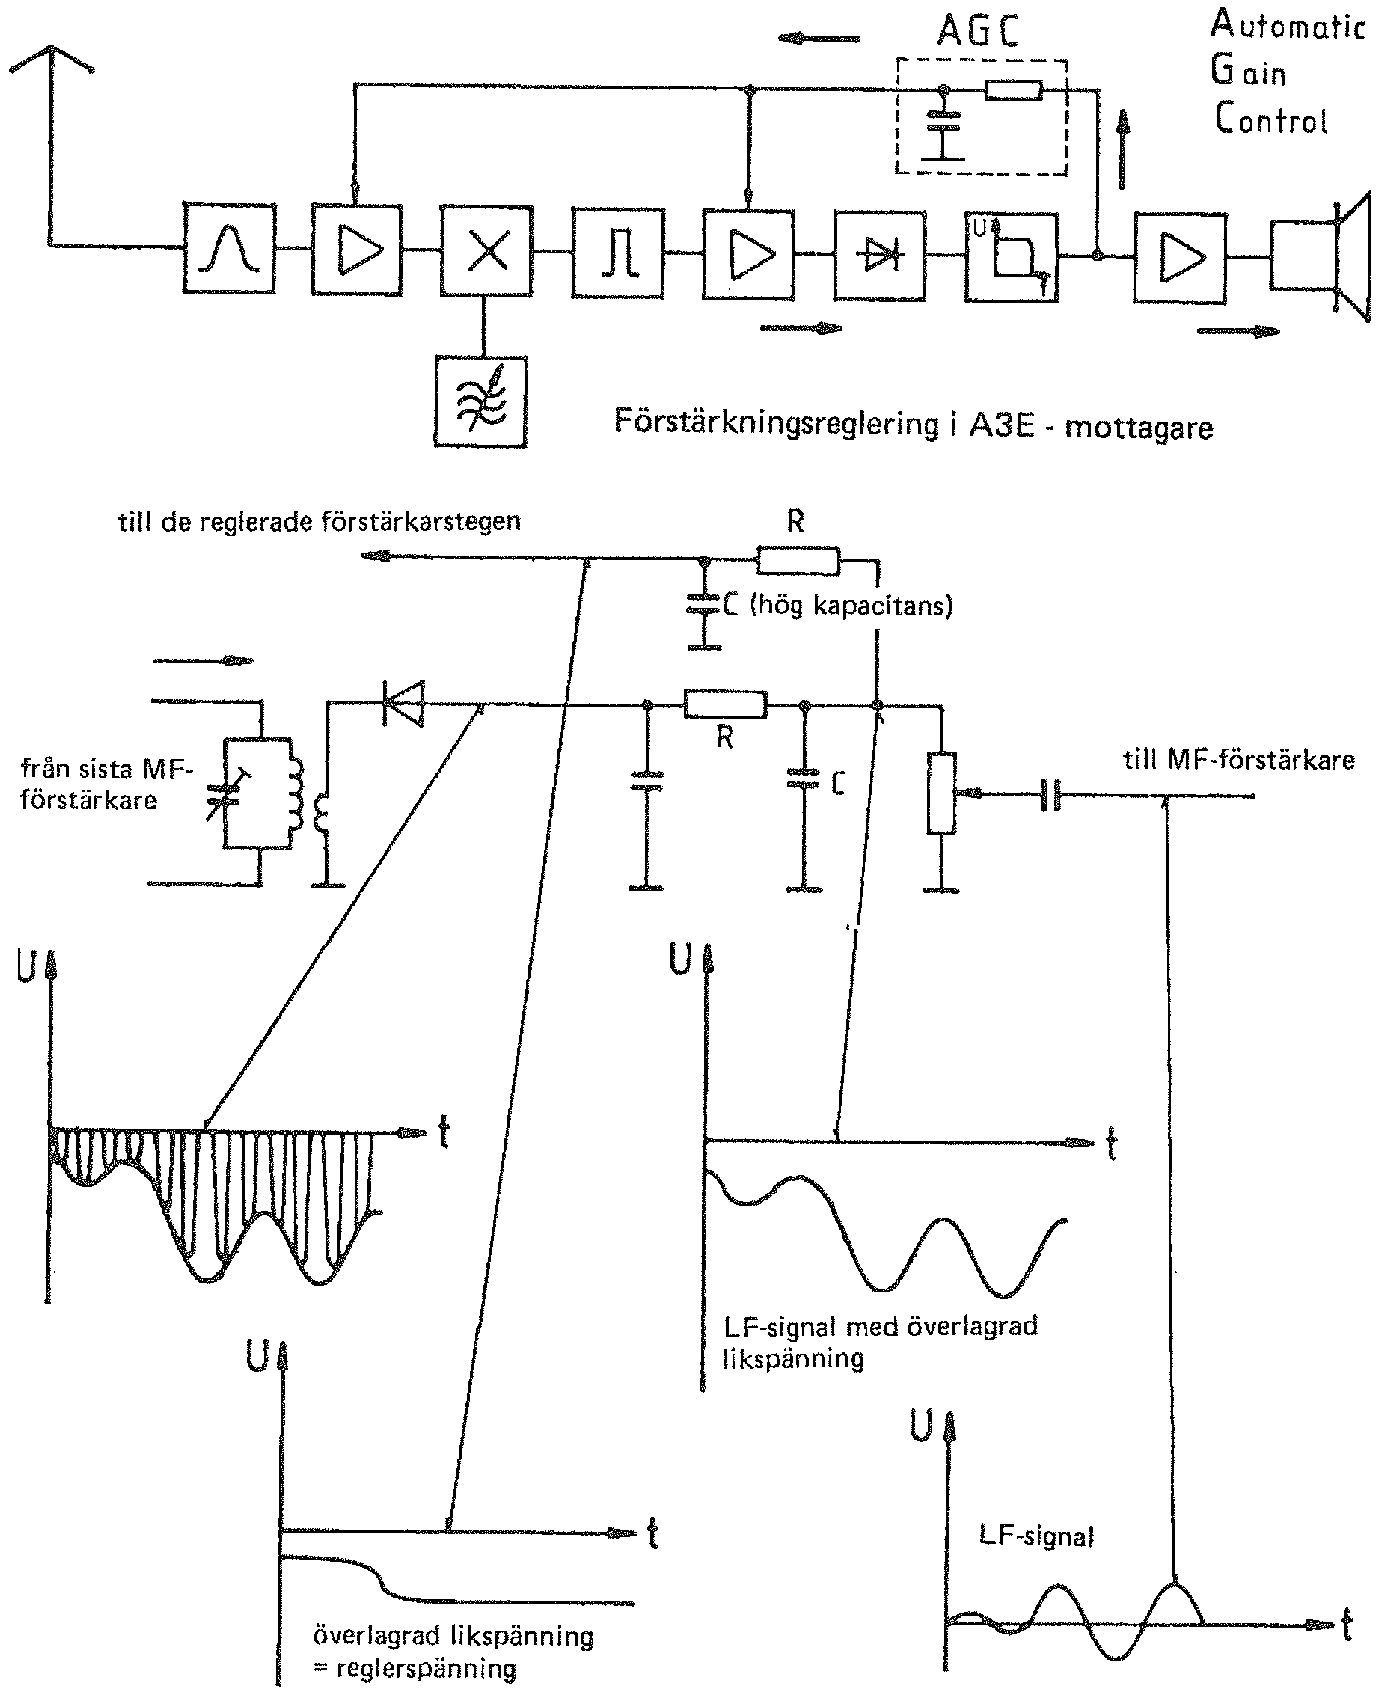
\includegraphics[width=\textwidth]{images/bild_2_4-20}
  \caption{AGC vid AM-mottagning med superheterodynmottagare}
  \label{fig:bildII4-20}
\end{figure}

Bild \ref{fig:bildII4-20}

Den likspänning som uppstår vid demoduleringen av MF-signalen i en
AM-mottagare används till förstärkningsreglering -- AGC. Den
LF-spänning som är överlagrad på likspänningen undertrycks i ett
RC-lågpassfilter. Likspänningen över kondensatorn följer variationerna
i den mottagna signalens styrka med en tidskonstant av ca 0.1~sekunder.
Likspänningen blir alltså inte påverkad av de betydligt snabbare
spänningsändringarna som kommer av moduleringen.

En stark bärvågssignal alstrar en hög likspänning och en svag signal
en låg likspänning, oberoende av moduleringen. Denna likspänning
återförs till de framförliggande HF- och MF-förstärkarstegen, vilka är
gjorda så att en hög reglerspänning sänker förstärkningen, medan en
låg spänning tillåter en hög förstärkning.

På så sätt kommer signalstyrkan efter de reglerade stegen att hållas
konstant samtidigt som mottagarens ingång inte överstyrs.

Den likspänning som filtrerats fram från detektorn kallas
reglerspänning eller AGC-spänning. Diodens polarisering är inte viktig
för att få ut LF vid demoduleringen, men däremot för att få rätt
polaritet på AGC-spänningen. i de flesta mottagare används negativ
AGC-spänning.

\subsection{AGC vid SSB (J3E)}
\index{SSB}
\index{AGC}

Bild \ref{fig:bildII4-21}

I de flesta utföranden lämnar produktdetektorn en växelspänning utan
överlagrad likspänning. Reglerspänningen alstras därför genom
likriktning av MF-spänningen med hjälp av en separat demoduleringsdiod
eller genom likriktning av LF-växelspänningen.

Vid SSB alstras det ju ingen MF-spänning under talpauserna, eftersom
ingen bärvåg tas emot då.
Tidskonstanten på lågpassfiltret för reglerspänningen måste därför vara längre
än vid AM, d.v.s. 0,5 till 2~sekunder.
En alltför snabb tillbakagång i reglerspänningen p.g.a. en för kort
tidskonstant skulle leda till mer mottagningsbrus i talpauserna.
I moderna mottagare finns det ofta en omkopplare för olika tidskonstanter.

Bild \ref{fig:bildII4-21}

\subsection{AGC vid CW (A1A)}
\index{CW}
\index{AGC}

Metoden för att alstra AGC-spänning är samma vid CW och SSB.

\subsection{AGC vid FM (F3E)}
\index{FM}
\index{AGC}

FM-mottagare brukar inte regleras av den anledningen att det vid FM
inte finns någon information i signalamplituden, utan finns i stället
i frekvensvariationerna i signalen.

\begin{figure}
  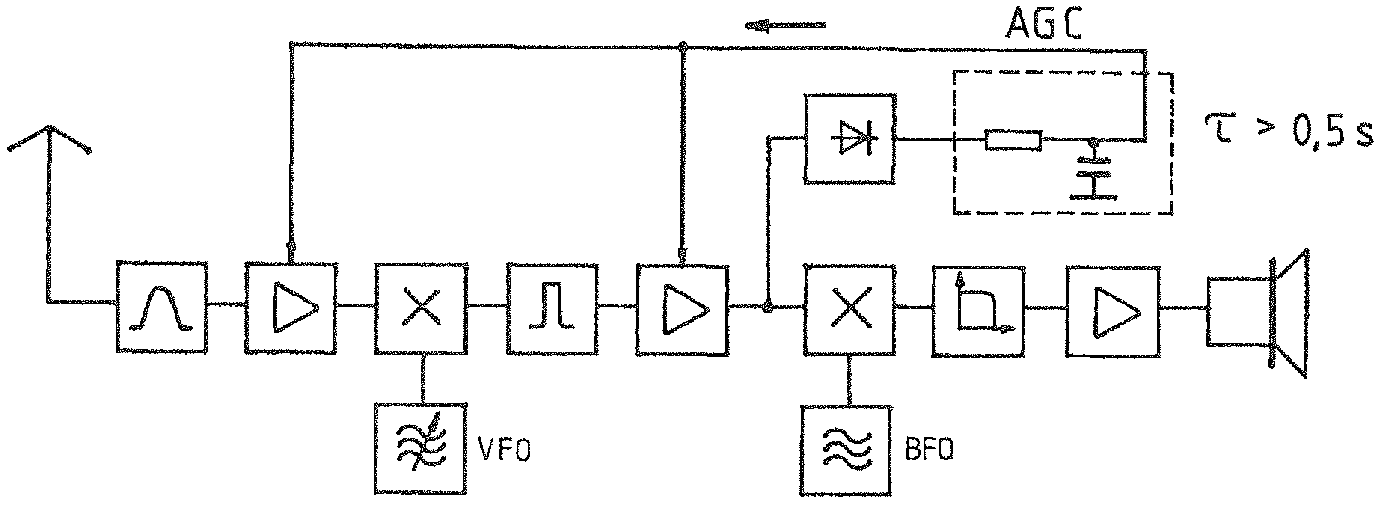
\includegraphics[width=\textwidth]{images/bild_2_4-21}
  \caption{AGC vid SSB- och CW-mottagning med superheterodynmottagare}
  \label{fig:bildII4-21}
\end{figure}

Helt avsiktligt läggs därför förstärkningen i mottagaren så, att en
sinussignal blir en kantvåg p.g.a. överstyrning i
förstärkarstegen. Ett eller flera sådana amplitudbegränsande steg,
även kallat ''limiter'', placeras före demoduleringssteget. Störningar
av amplitudvariationer kommer då att klippas bort och inte störa
mottagningen.

Störande signaler inom nyttobandbredden har dock ingen större inverkan
så länge som den önskade signalens styrka är en halv s-enhet större än
den störande signalens styrka. Likaså försvinner det störande bruset
vid mottagning av en FM-sändare mycket snabbt över denna signalnivå.
Amplitudmodulerade störningar, som t.ex. de från tändgnistor i
förbränningsmotorer, har liten påverkan vid tillräckligt stark
nyttosignal.

\subsection{Signalstyrkemätare (S-meter)}
\textbf{HAREC a.\ref{HAREC.a.4.3.9}\label{myHAREC.a.4.3.9}}
\index{signalstyrkemätare}
\index{mottagare!signalstyrkemätare}
\index{S-meter}
\index{mottagare!S-meter}

AGC-spänningen i en mottagare för AM, CW och SSB kan även styra en
S-meter, som ger besked om hur stark signalen in i mottagaren är. (Se
Appendix \ref{s-enhet}.)

\subsection{Brusspärr}
\textbf{HAREC a.\ref{HAREC.a.4.3.10}\label{myHAREC.a.4.3.10}}
\index{brusspärr}
\index{mottagare!brusspärr}
\index{squelch}
\index{mottagare!squelch}

I en FM-mottagare hörs bara brus när det inte kommer in en
tillräckligt stark signal.  Bruset är genomträngande eftersom
FM-mottagare arbetar med hög förstärkning. En \emph{brusspärr}
(eng. \emph{squelch})
är en anordning som stoppar signalerna till LF-förstärkaren när
signalerna ej uppnår en viss nivå. På så sätt slipper man att höra på
bruset. I mottagare för flera sändningsslag och därför även AGC kan
denna funktion styra brusspärren, men i en ren FM-mottagare arbetar
MF-förstärkarna utan AGC. I det fallet behövs någon annan anordning för
att skilja mellan en modulerad signal och brus. Ofta finns ett reglage
(squelch) för hur stark signalen ska vara innan spärren öppnar.
